\section{Nuclear deformations}
\label{sec:deformations}
We shall now give a description of the nuclear shape in a formal framework. We will start by expanding the nuclear radius in terms of spherical harmonics, so that we can truncate and omit terms to describe certain configurations of the nucleus, so that we are able to illustrate the simple case of an axial quadrupole deformation. After that, we will briefly discuss the more general case of trixial, octupole, and parity breaking configurations.
\subsection{Quadrupole deformation}
Assuming the nuclear volume to be evaluated as
\begin{equation}
    V(A) = \frac{4}{3}\pi R^3
\end{equation}
Let us suppose to consider variations of the nuclear radius $R$ in terms of spherical harmonics
\begin{equation}
    R(\theta, \phi) = R_0\bigg[1+\sum_{\lambda \mu}\alpha_{\lambda \mu}\,Y_{\lambda\mu}(\theta,\phi)\bigg]
\end{equation}
where the moments $\alpha_{\lambda \mu}$ defined as
\begin{equation}
    \alpha_{\lambda \mu}=\int Y_{\lambda\mu}^*(\theta, \phi)R(\theta, \phi) d\Omega
\end{equation}
are considered small, in the sense that $|\alpha_{\lambda \mu}| ^2 \ll |\alpha_{\lambda \mu}| $. We have that $Y_{00}$ is constant, so its moment does not produce an interesting variation. We can set $\alpha_{00}=0$. 
Since $Y_{10}$, $Y_{11}$ and $Y_{1-1}$ are odd for $\theta + \pi$ and $\phi + \pi$, we have that $\alpha_{1\mu}$ vanishes in a reference frame in which the centre of mass is at the origin.
\\Now, let us consider only $\alpha_{2\mu}$ coefficients and neglect higher degree terms, so that the deformation is purely quadrupolar, then the radius reads
\begin{equation}
    R(\theta, \phi) = R_0\bigg[1+\sum_{\mu=-2}^2\alpha_{2\mu}\,Y_{2\mu}(\theta, \phi)\bigg].
\end{equation}
If we assume to be in the reference frame in which the inertia tensor, proportional to the coefficients $\alpha_{2\mu}$, is diagonal, which is known as intrinsic frame, then the sum 
\begin{equation*}\alpha_{21}Y^*_{21} + \alpha_{2-1}Y^*_{2-1}\end{equation*} vanishes. Since $R$ is a real valued function, we have the relation
\begin{equation}
\alpha_{\lambda \mu}Y_{\lambda\mu}+\alpha_{\lambda -\mu}Y_{\lambda-\mu}=2\Re{\alpha_{\lambda \mu}Y_{\lambda\mu}},
\end{equation}
as a consequence, the resulting expansion reads
\begin{align}
    R(\theta, \phi) &= R_0\bigg[1+a_{20}Y_{20}+2\Re{a_{22}Y_{22}}\bigg]\nonumber
    \\&=R_0\bigg[1+\sqrt{\frac{5}{16\pi}}\bigg(a_{20}(3\cos^2\theta-1)+ 2a_{22}\sqrt{3}\sin^2\theta(\cos^2\phi-\sin^2\phi) \bigg)\bigg].
\end{align}
If we perform the substitution 
\begin{align}
    \label{eq:a20}
    a_{20} &= \beta\cos(\gamma)
    \\  a_{22} &= \beta\sin(\gamma)\label{eq:a22}
\end{align} 
and express the variation of $R$ along the cartesian axes, we get 
\begin{align}
     R_x - R_0  =\delta R_{x}&=\sqrt{\frac{5}{4\pi}}\beta R_0 \cos\bigg(\gamma - \frac{2\pi}{3}\bigg),
    \\R_y - R_0 =\delta R_{y}&=\sqrt{\frac{5}{4\pi}}\beta R_0 \cos\bigg(\gamma + \frac{2\pi}{3}\bigg),
    \\R_z - R_0 =\delta R_{z}&=\sqrt{\frac{5}{4\pi}}\beta R_0 \cos\gamma.
\end{align}
Assuming the value of $\beta$ to always be positive, in the case $\gamma=0$, $\delta R_x = \delta R_y <\delta R_z$, meaning the nucleus is in a \textit{prolate} configuration; while in the case of $\gamma = \pi/3$, $\delta R_x = \delta R_y > \delta R_z$, meaning the nucleus has an \textit{oblate} shape. A general convention is to write $\beta$ with a negative sign in the oblate case, and a positive sign in the prolate case.
\\By using trigonometric identities, it is trivial to show that unique shapes are found only for $\gamma\in [0; \pi/3]$, if $\gamma$ takes a value different from $0$ or $\pi/3$, the shape is said to be triaxial, meaning $\delta R_z \neq \delta R_x \neq \delta R_y$, the nucleus has no more rotational symmetries and is only symmetric for reflections along the $(x, y)$, $(x, z)$ and $(y, z)$ planes, which also induces parity symmetry.
\subsection{Nilsson model}
To understand the effect on single-particle motion of a deformed potential, we can consider the case of an axially deformed harmonic oscillator potential, for which $ \omega_z \neq \omega_x = \omega_y = \omega_\perp$, meaning the oscillator frequency takes on a different value on the $z$ axis than in the $x$ and $y$ axes.
\\To treat the deformation perturbatively, we can assume that the various frequencies deviate from the unperturbed $\omega_0=41/A^{1/3}$ MeV, in which case they may read
\begin{align}
\omega_z = \omega_0 - \frac 2 3 \varepsilon,\\
\omega_\perp = \omega_0 + \frac 1 3 \varepsilon,
\end{align}
this definition of the frequencies satisfies the conservation of volume, at lowest order in $\varepsilon$, assumed to hold for 
\begin{equation}
    \label{eq:volume_cons}
    \omega_0 ^ 3 = \omega_z \omega_\perp^2.
\end{equation}
We can thus write the single-particle Hamiltonian in the deformed potential as
\begin{align}
    H&=H_0 +\varepsilon H_1,\\
    H_0 &= -\frac{\hbar^2}{2m}\nabla^2 + \frac 1 2 m \omega_0^2 r^2,\\
    \varepsilon H_1 &= \frac 1 3 \omega_0 ^2 \varepsilon (x^2 + y^2 -2z^2) = -\frac 1 3 \sqrt{\frac{16\pi}{5}}m\omega_0^2\varepsilon r^2 Y_{20}.
\end{align}
$H_0$ is the usual spherical harmonic potential, for which the eigenfunctions, expressed through the usual quantum numbers $\ket{nljm_j}$ are known. Assuming $\varepsilon$ to be small, we can evaluate the first order correction of $H_1$ to the system, which reads
\begin{align}
\Delta E &= \bra{nljm_j}\varepsilon H_1 \ket{nljm_j},
\\&= -\frac 1 3 \sqrt{\frac{16 \pi}{5}}\varepsilon m \omega_0^2 \int r^2 u_{nl}(r)\bra{jm_j} Y_{20}\ket{jm_j} dr,
\\&= \frac \varepsilon 6 m\omega_0^2 \int r^2 u_{nl}(r)\frac{3m_j^2 - j(j+1)}{j(j+1)}dr,
\end{align}
thus in the limit of large $j$, states with the maximum total angular momentum projection $m_j$ are shifted upwards, while states with the minimum $m_j$ are shifted downwards; moreover, eigenstates with $\pm m_j$ are degenerate, as expected by the reflection symmetry of the Hamiltonian if the $z$ axis is inverted.
Adding further empirical terms to reproduce experimental data, and the spin-orbit coupling, results in the formulation of the Nilsson model \cite{nilsson}. In figure \ref{fig:nilsson}, a graphical representation of the energy levels in the Nilsson model is shown \cite{wikipedia_equation_of_state}.
\begin{figure}[H]
    \centering
    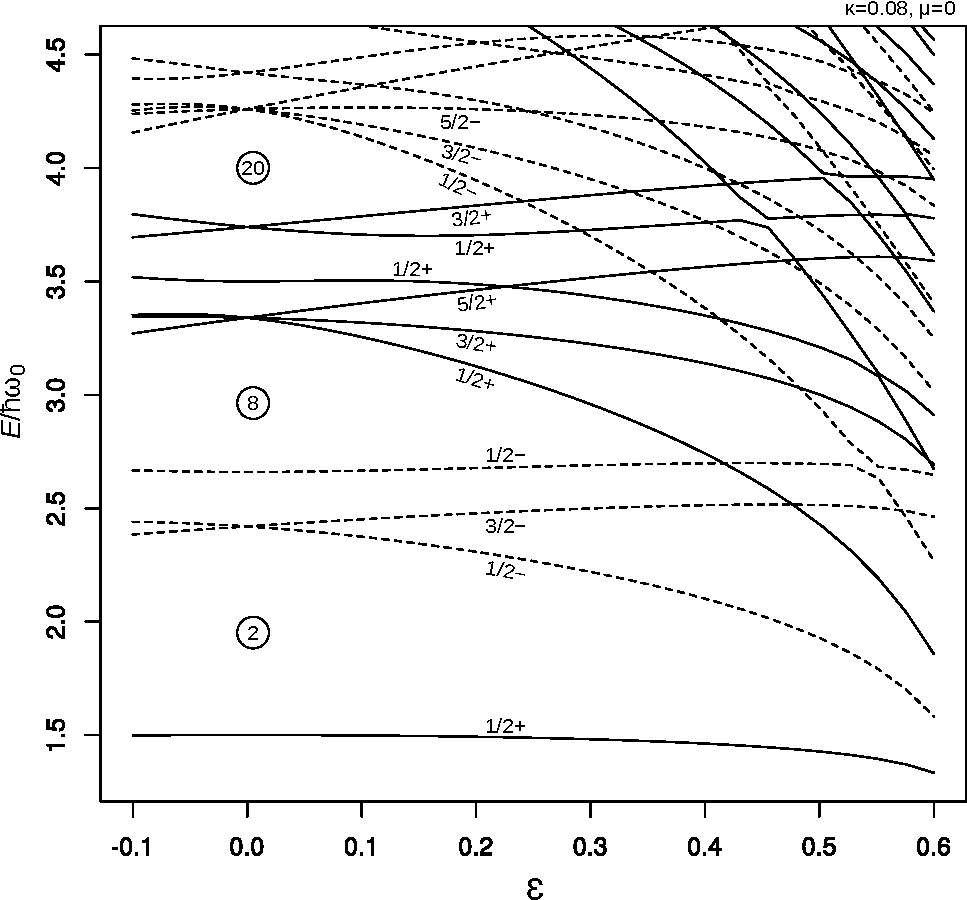
\includegraphics[width=0.7\textwidth]{Images/nilsson.pdf}
    \caption{Nilsson model energy levels trends, as a function of $\varepsilon$.}
    \label{fig:nilsson}
\end{figure}
\subsubsection{Deformed Woods-Saxon}
Recent studies of deformed nuclei have been carried out using empirical potentials such as deformed Woods-Saxon potentials \cite{def_WS_dudek,defWSfissionbarriers}. In these models, the nuclear shape is expanded as 
\begin{equation}
R(\theta) = R_0\bigg[1+\sum_{\lambda}^L \beta_{\lambda}Y_{\lambda 0}\bigg],
\end{equation}
so that the solution is axially symmetric and the problem is reduced to just the $(r, \theta)$ coordinates, in which we can write the potential as
\begin{equation}
    \label{eq:def_WS}
    U_\text{WS}(r, \theta) = -\frac{U_0(A, N)}{1+e^\frac{r - R(\theta)}{a}}.
\end{equation}
\subsection{Octupole deformations and parity breaking}
While quadrupole deformations concern nuclei across the whole chart, octupole deformations are much less common, being found only in heavier nuclei.
Under the parity operation $\mathcal P: \bm r \mapsto -\bm r$, coefficients of the spherical harmonics transform as
\begin{equation}
    \mathcal P \alpha_{\lambda \mu} = (-1)^{\lambda} \alpha_{\lambda \mu},
\end{equation}
hence a nuclear octpuole deformation, whose degree $\lambda=3$, would break parity symmetry. In figure \ref{fig:octupole_defs} a graphical representation of the spherical harmonics for $\lambda=3$ and $\mu=0,2$ is shown.
\begin{figure}[H]
    \centering
\begin{minipage}{0.48\textwidth}
    \centering
    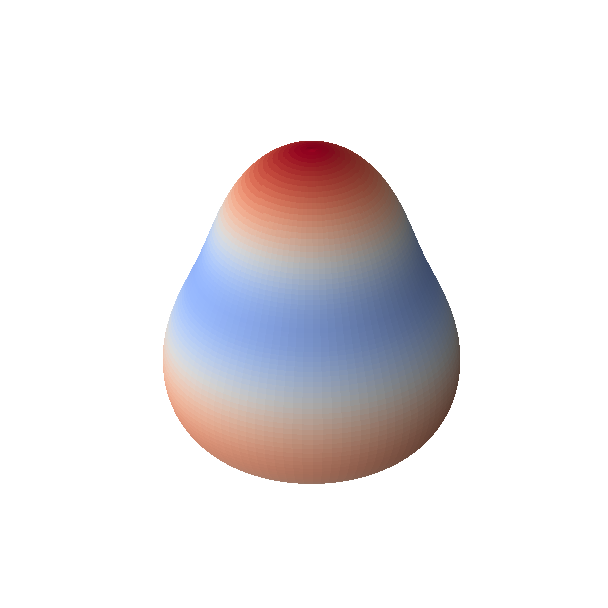
\includegraphics[width=\textwidth]{Images/octupole_Y30}
  \end{minipage}
  \hfill
  \begin{minipage}{0.48\textwidth}
    \centering
    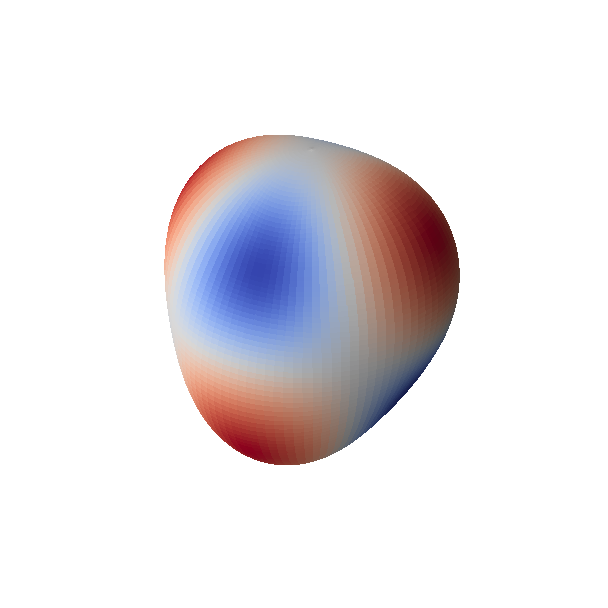
\includegraphics[width=\textwidth]{Images/octupole_Y32}
  \end{minipage}
    \caption{Graphical representation of possible octupole deformations. On the left, the axially symmetric $Y_{30}$ deformation, on the right, the non-axial octupole deformation $Y_{32}$.}
    \label{fig:octupole_defs}
\end{figure}




